% Compact UC3M template, for documents with very little room (one-page
% summaries, short hand-ins, etc.). English version of main.tex: same
% package, same layout; the only change is the babel line below. Demo of
% the minimal title block, compact sections (with a "run-in"
% subsubsection), the \reference line, a list, a table and a figure.
% One-column version; see main-twocolumn.tex (Spanish) for the same
% package in two-column mode.
%
% Build:  make      (latexmk -lualatex, produces build/main-en.pdf along
%                    with the Spanish demos)
%
% No inputenc/fontenc needed: under LuaLaTeX+fontspec the engine handles
% the encoding.
\documentclass[10pt]{article}

% babel goes BEFORE uc3mtight: the package loads hyperref internally, and
% hyperref needs babel already active to pick the right \autoref names.
% The package has no language option: it detects whether babel is set to
% Spanish and only then applies its babel-spanish tweaks; with english (or
% no babel at all) everything is left as LaTeX/babel provide it.
\usepackage[english]{babel}
\usepackage{uc3mtight}

\title{Summary: result caching in the query layer}
\subject{Databases}
\group{Group 84}
\author{Raúl Aguilar Arroyo \and Ana Pérez Ruiz}
\date{Academic year 2026/2027}
% Optional label defaults to "Reference" in English ("Referencia" in
% Spanish); pass one explicitly with \reference[Article]{...} to override.
\reference{A. Silberschatz, H. F. Korth and S. Sudarshan, \emph{Database
  System Concepts}, 7th ed., McGraw-Hill, 2019, ch.~13}

\begin{document}
\maketitle

\section{Motivation}

The cost of recomputing repeated queries over the same data set motivates
introducing a caching layer between the application and the database
engine, reducing perceived latency without modifying the underlying
schema.

\subsection{Approach}

We evaluate an in-memory LRU cache placed in front of the relational
engine, explicitly invalidated on every write to the affected tables.

\subsubsection{Scope} This summary covers only read-only queries over a
single table; multi-table joins are outside the analysis presented here.

\section{Results}

\autoref{tab:results} summarises the latency reduction observed for
different cache sizes.

\begin{table}[h]
  \centering
  \caption{Mean latency by cache size.}
  \label{tab:results}
  \begin{tabular}{@{}lrr@{}}
    \toprule
    Cache size & Latency (ms) & Hit rate (\%) \\
    \midrule
    No cache & 42 & --- \\
    128 entries & 19 & 61 \\
    512 entries & 8 & 89 \\
    \bottomrule
  \end{tabular}
\end{table}

Observed advantages:
\begin{itemize}
  \item Mean latency reduction above 80\,\% with 512 entries.
  \item No changes to the schema or to the application's queries.
\end{itemize}

\autoref{fig:latency} illustrates the trend.

\begin{figure}[h]
  \centering
  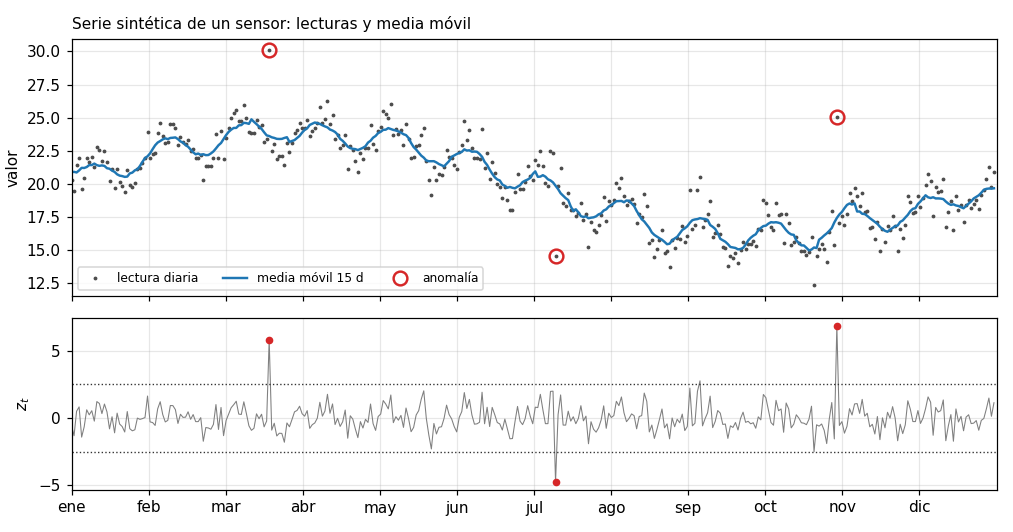
\includegraphics[width=\linewidth]{figs/demo-figura}
  \caption{Mean latency as a function of cache size.}
  \label{fig:latency}
\end{figure}

\section{Conclusion}

A simple LRU cache, invalidated on write, delivers a substantial latency
reduction at a low implementation cost, provided that queries are limited
to single-table reads.

\end{document}
